% !TEX root = ../main.tex
\section{Controllability-prinsippet}\label{thr:controllability-principle}

\paragraph{Definisjon.} Controllability-prinsippet sier at en leder kun skal evalueres og belønnes på utfall hun selv kan kontrollere. Utfall som er drevet av faktorer utenfor lederens beslutningsrom (eksogene markedssvingninger, andre divisjoners adferd, makroforhold) skal filtreres bort fra prestasjonsmålet. [SLIDE]

\subsection*{Forklaring}

Prinsippet er et normativt rettferdighets- og effektivitetskrav: hvis lederen straffes eller belønnes for variasjon hun ikke har innvirkning på, blir signalet i prestasjonsmålet støyete og insentivene svekkes. Risikoaverse ledere må også kompenseres med høyere lønn for å bære ikke-kontrollerbar risiko (jf.\ \thref{informativeness-principle}{informativeness-principle}), noe som gjør slike kontrakter dyre for prinsipalen. Prinsippet ligger bak hele inndelingen i \thref{responsibility-centers}{responsibility centers} -- man skreddersyr måltallet til lederens faktiske kontrollvariabler. [SLIDE/BOK]

I praksis er ikke skillet mellom kontrollerbart og ikke-kontrollerbart skarpt. En divisjonsleder kontrollerer ikke valutakurser direkte, men kan velge å sikre seg mot dem. En produksjonssjef kontrollerer ikke råvarepriser, men kan velge leverandører. Anvendelse av prinsippet krever derfor en konkret vurdering av \emph{hvilken type} kontroll lederen reelt har. [BOK]

\subsection*{Kjerneforutsetninger}
\begin{itemize}
\item Det er mulig å skille kontrollerbare fra ikke-kontrollerbare faktorer i målingen (regnskapsmessig eller analytisk).
\item Lederen er risikoaversiv -- ellers ville hun gjerne tatt på seg ukontrollerbar risiko gratis.
\item Informasjonen om hva som er kontrollerbart er rimelig symmetrisk; ellers oppstår diskusjon om hva som egentlig var ``utenfor lederens kontroll''.
\end{itemize}

\subsection*{Muligheter}
\begin{itemize}
\item Gir grunnlag for å velge \emph{riktig centertype} ut fra lederens beslutningsrettigheter.
\item Reduserer kompensasjon for risiko -- billigere insentivkontrakter.
\item Reduserer demotivering: ledere som ``rammes'' av ukontrollerbare svingninger gir opp innsats (locus of control-effekt).
\item Begrunner bruk av \emph{relative performance evaluation} (sammenligning mot peers) for å filtrere ut bransje-/makrostøy.
\end{itemize}

\subsection*{Begrensninger og kritikk}
\begin{itemize}
\item Strikt anvendelse kan fjerne all risikodeling -- men noen ganger \emph{ønsker} prinsipalen at lederen bærer risiko (eierperspektiv, langsiktig hensyn).
\item Mange utfall er delvis kontrollerbare. Hvor settes grensen?
\item Lederen kan strategisk omklassifisere dårlige resultater som ``ikke-kontrollerbart'' (\emph{ex-post excuse}) og gode som ``mitt verk''.
\item Prinsippet sier ikke noe om hvilket \emph{nivå} av målet som er riktig (gaming, ratchet-problemer ligger fortsatt der).
\item I virkeligheten ønsker eier ofte at ledere tar ansvar utover egen kontroll -- f.eks.\ CEO som påvirker selskapets evne til å håndtere kriser de ikke skapte selv.
\end{itemize}

\subsection*{Modell / illustrasjon}

\begin{figure}[H]
\centering
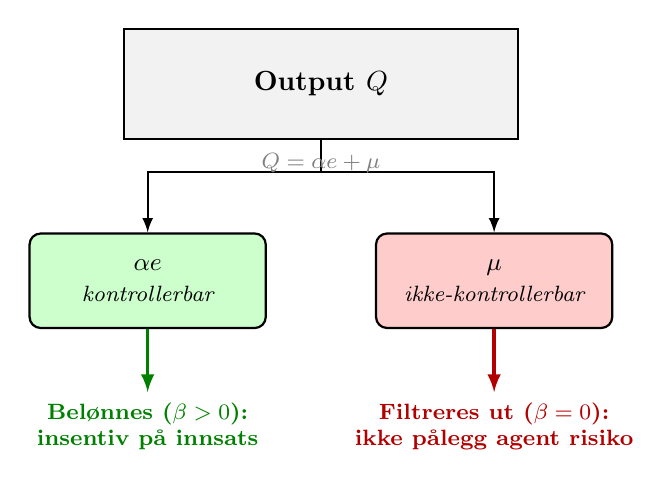
\begin{tikzpicture}[>=latex, every node/.style={font=\small}]
  % Output Q (stor boks)
  \node[draw, thick, fill=gray!10, minimum width=5.0cm, minimum height=1.4cm, font=\bfseries] (Q) at (0,3) {Output $Q$};
  % Dekomponering: alpha*e + mu
  \node[draw, rounded corners, thick, fill=green!20, minimum width=3.0cm, minimum height=1.2cm, align=center] (E) at (-2.2,0.5) {$\alpha e$\\ \footnotesize\itshape kontrollerbar};
  \node[draw, rounded corners, thick, fill=red!20, minimum width=3.0cm, minimum height=1.2cm, align=center] (M) at (2.2,0.5) {$\mu$\\ \footnotesize\itshape ikke-kontrollerbar};
  % Piler fra Q til dekomp
  \draw[->, thick] (Q.south) -- ++(0,-0.4) -| (E.north);
  \draw[->, thick] (Q.south) -- ++(0,-0.4) -| (M.north);
  \node[font=\footnotesize, gray] at (0,2.0) {$Q = \alpha e + \mu$};
  % Pil ned til β-beslutning
  \draw[->, very thick, green!50!black] (E.south) -- ++(0,-0.8)
    node[below, font=\footnotesize\bfseries, align=center] {Belønnes ($\beta > 0$):\\ insentiv på innsats};
  \draw[->, very thick, red!70!black] (M.south) -- ++(0,-0.8)
    node[below, font=\footnotesize\bfseries, align=center] {Filtreres ut ($\beta = 0$):\\ ikke pålegg agent risiko};
\end{tikzpicture}
\caption{\textbf{Controllability-prinsippet.} Mål agenten på den delen av $Q$ hun \emph{kontrollerer} ($\alpha e$), og filtrer bort det hun \emph{ikke} kontrollerer ($\mu$ -- markedssjokk, valuta, peer-firmaer). I praksis: bruk relative måltall, ekskluder ekstraordinære poster, eller dekomponer KPI-er. Strikt anvendelse senker risikopremien uten å svekke insentivet. [SLIDE -- BSZ kap.\ 10]}
\end{figure}

I prinsipal-agent-modellen $W = W_0 + \beta Q$ er $Q$ et målt prestasjonstall. Controllability-prinsippet sier at vekten $\beta$ bør være null på komponenter i $Q$ som lederen ikke kontrollerer, og positiv kun på komponenter hun \emph{kan} påvirke. Tilsvarende: når støyen i $Q$ øker, må $W_0$ (fast lønn) opp og $\beta$ ned (informativeness-prinsippet).

\begin{center}
\begin{tabular}{@{}lll@{}}
\toprule
\textbf{Kontroll lederen har} & \textbf{Egnet centertype} & \textbf{Måltall} \\
\midrule
Kun input-mix (output gitt) & Cost center & Kostnad pr.\ enhet \\
Kun aktivitetsnivå & Expense center & Budsjettoverholdelse \\
Salgsinnsats, kundekontakt & Revenue center & Omsetning \\
Pris, mix, kostnad & Profit center & Profit \\
Profit + investeringer & Investment center & ROA, EVA \\
\bottomrule
\end{tabular}
\end{center}

\subsection*{Eksempler}
\begin{itemize}
\item \textbf{SAS:} Flight crew kan ikke holdes ansvarlig for drivstoffpris-svingninger. Crew evalueres på punktlighet og kundeservice (kontrollerbart), ikke drivstoffmargin (ikke-kontrollerbart). [EKS]
\item \textbf{Equinor:} Lete-avdelingen evalueres på funnrate og kostnad pr.\ funn, ikke på oljeprisen, fordi prisen er global og eksogen. [EKS]
\item \textbf{Norsk Hydro:} Aluminium-divisjonene har historisk hatt resultatregnskap justert for aluminiumspris (LME-pris) for å isolere driftsbidraget fra prissyklusen. [EKS]
\end{itemize}

\subsection*{Kobling til søyle og andre teorier}
Søyle: \STwo\ primært, men direkte koblet til \SThree\ (kompensasjon) og \SOne\ (beslutningsrett $=$ det som er kontrollerbart). Relatert: \thref{responsibility-centers}{Responsibility centers}, \thref{informativeness-principle}{Informativeness-prinsippet}, \thref{absolute-vs-relative-performance}{Relative performance evaluation}.

\paragraph{Brukt i spørsmål:} Q01, Q05, Q10, Q14.
